\documentclass[a5paper,headsepline,titlepage,10pt,nnormalheadings,DIVcalc]{scrbook}
\usepackage[a5paper,backref]{hyperref}
%\usepackage{palatino}
\usepackage{graphicx}
\usepackage{wrapfig}
\usepackage[bahasa]{babel}
\usepackage{fancyhdr}
\usepackage{pstricks}
%\setlength{\voffset}{0.5in}
%\setlength{\oddsidemargin}{28pt}
%\setlength{\evensidemargin}{0pt}
\renewcommand{\footrulewidth}{0.5pt}
\lhead[\fancyplain{}{\thepage}]%
      {\fancyplain{}{\rightmark}}
\rhead[\fancyplain{}{\leftmark}]%
      {\fancyplain{}{\thepage}}
\pagestyle{fancy}
\lfoot[\emph{Ziarah Gua Maria Rosa Mystica Tuntang}]{}
\rfoot[]{\emph{Lingkungan St Petrus Maguwo}}
\cfoot{}

\newcommand{\BU}[1]{\begin{itemize} \item[U:] #1 \end{itemize}}
\newcommand{\BI}[1]{\begin{itemize} \item[I:] #1 \end{itemize}}
\newcommand{\BP}[1]{\begin{itemize} \item[P:] #1 \end{itemize}}
\newcommand{\kamiMenyembah}{\BP{ Kami menyembah Dikau ya Tuhan dan bersyukur\\kepadaMu.}
\BU{ Sebab dengan salib suciMu, Engkau telah menebus dunia.}
}
\newcommand{\kasihanilahKami}{\BP{Yesus, yang paling taat, lemah lembut dan rendah hati, kasihanilah kami.}
\BU{Allah ampunilah kami orang berdosa.}}
\title{Jalan Salib\\Berdasarkan Refleksi Yesus}
\author{Ziarah Gua Maria Rosa Mystica Tuntang\\Lingkungan St. Petrus Maguwo}
\date{31 Oktober 2010}
\hyphenation{a-kan}
\hyphenation{ba-gi-mu}
\hyphenation{ber-a-da}
\hyphenation{ber-du-a}
\hyphenation{be-ri-kan}
\hyphenation{ber-ka-ta}
\hyphenation{ber-nya-nyi}
\hyphenation{ber-sa-ma}

\hyphenation{dah-syat}
\hyphenation{DA-RAH-KU}
\hyphenation{da-tang}
\hyphenation{di-ka-ta-kan}
\hyphenation{di-pim-pin}
\hyphenation{di-se-rah-kan}
\hyphenation{di-tum-pah-kan}

\hyphenation{Eng-kau}
\hyphenation{ha-dap-an}
\hyphenation{han-tar-kan-lah}
\hyphenation{ha-rap-an}

\hyphenation{ja-lan}
\hyphenation{ja-ngan-lah}

\hyphenation{ka-nak}
\hyphenation{ka-re-na}
\hyphenation{kau-lim-pah-kan}
\hyphenation{Kau-cip-ta-kan}
\hyphenation{ke-bang-kit-an-Nya}
\hyphenation{ke-da-tang-an}
\hyphenation{ke-da-tang-an-Nya}
\hyphenation{ke-dua}
\hyphenation{ke-na-ik-kan-nya}
\hyphenation{ke-pa-daMu}
\hyphenation{ke-ra-him-an}
\hyphenation{ke-se-jah-te-ra-an-mu}
\hyphenation{ko-men-tar}

\hyphenation{la-ma-nya}
\hyphenation{lim-pah-kan}

\hyphenation{ma-nu-sia}
\hyphenation{me-nga-da-kan}
\hyphenation{me-ngan-dung-lah}
\hyphenation{me-ngu-kuh-kan}
\hyphenation{me-la-lui}
\hyphenation{me-lim-pah-kan}
\hyphenation{me-lu-hur-kan}
\hyphenation{me-me-cah-me-cah-kan}
\hyphenation{mem-per-sem-bah-kan}
\hyphenation{me-nan-da-ta-ngan-i}
\hyphenation{men-cin-tai}
\hyphenation{meng-a-lir-kan}
\hyphenation{me-nga-sihi}
\hyphenation{me-nge-lu-ar-kan}
\hyphenation{meng-u-cap-kan}
\hyphenation{meng-ung-kap-kan}
\hyphenation{me-num-buh-kan}
\hyphenation{me-nya-ta-kan}
\hyphenation{me-nye-la-mat-kan}
\hyphenation{me-nye-rah-kan}
\hyphenation{me-nye-rah-kanNya}
\hyphenation{me-ra-ya-kan}

\hyphenation{o-rang}
\hyphenation{o-rang-o-rang}

\hyphenation{pa-sang-kan-lah}
\hyphenation{pa-tut}
\hyphenation{pe-ne-ri-ma-an}
\hyphenation{pe-ngam-pun-an}
\hyphenation{Pe-ngan-ta-ra}
\hyphenation{peng-hi-bur-an}
\hyphenation{per-bu-at-an-nya}
\hyphenation{per-ka-ta-an}
\hyphenation{per-ka-win-an}
\hyphenation{per-ni-kah-an}
\hyphenation{per-se-ku-tu-an}
\hyphenation{per-sem-bah-an}
\hyphenation{rom-bong-an}

\hyphenation{se-la-ma}
\hyphenation{se-ka-li-an}
\hyphenation{se-pan-jang}
\hyphenation{se-ra-ya}
\hyphenation{Su-dar-yan-to}

\hyphenation{te-ta-pi}
\hyphenation{ta-ngan-Mu}
\hyphenation{Tu-han}
\hyphenation{tu-lang}
\hyphenation{tu-lang-tu-lang}

\hyphenation{u-mat-Mu}
\hyphenation{wa-kil}

\hyphenation{ba-gi-mu}
\hyphenation{di-se-rah-kan}
\hyphenation{me-la-lui}
\hyphenation{ka-nak}
\hyphenation{ka-re-na}
\hyphenation{ber-ka-ta}
\hyphenation{te-ta-pi}
\hyphenation{per-ka-win-an}
\hyphenation{pa-tut}
\hyphenation{me-lu-hur-kan}
\hyphenation{ber-nya-nyi}
\hyphenation{di-tum-pah-kan}
\hyphenation{pe-ngam-pun-an}
\hyphenation{ber-a-da}
\hyphenation{kau-lim-pah-kan}
\hyphenation{ke-bang-kit-an-Nya}
\hyphenation{per-ka-ta-an}
\hyphenation{pa-sang-kan-lah}
\hyphenation{DA-RAH-KU}
\hyphenation{ke-na-ik-kan-nya}
\hyphenation{per-sem-bah-an}
\hyphenation{per-se-ku-tu-an}



\begin{document}
%\maketitle
\thispagestyle{empty}
\newsavebox\IBox
\sbox\IBox{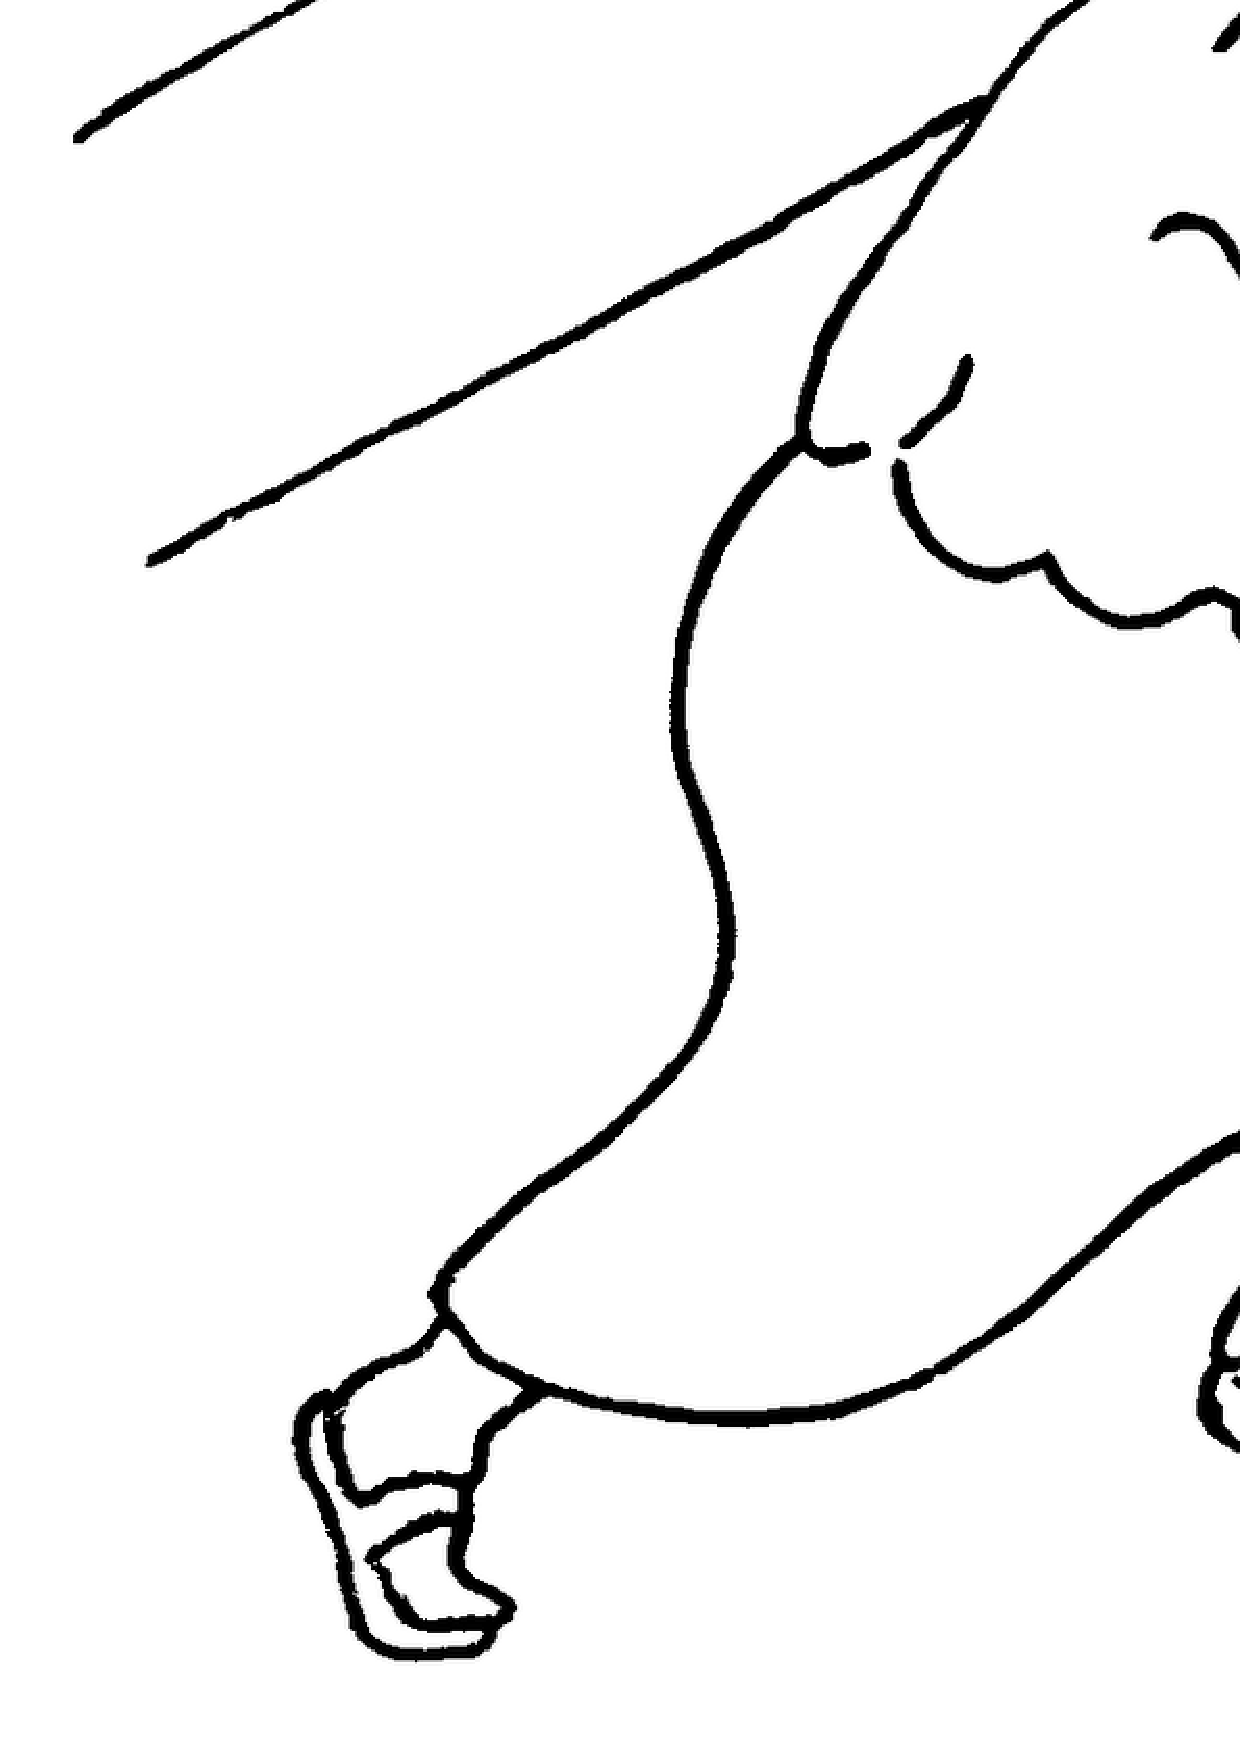
\includegraphics[scale=0.125]{cart017.png}}
% set up the picture environment
\psset{unit=1in}
\begin{center}
\begin{pspicture}(4in,6in)
% set up the fonts we use
\DeclareFixedFont{\PT}{T1}{ppl}{b}{it}{0.25in}
\DeclareFixedFont{\PTsmall}{T1}{ppl}{b}{it}{0.2in}
\DeclareFixedFont{\PTsmallest}{T1}{ppl}{b}{it}{0.15in}
\DeclareFixedFont{\PTtext}{T1}{ppl}{b}{it}{11pt}
\DeclareFixedFont{\Logo}{T1}{pbk}{m}{n}{0.15in}
% place the front cover picture
\rput[cb](2,2.5){\usebox\IBox}
% put the text on the front cover
\rput[cb](2,5.5){\PT {JALAN SALIB}}
\rput[cb](2,5.125){\PT {GUA MARIA ROSA MYSTICA}}
\rput[cb](2,4.85){\PTsmall {Tuntang Salatiga}}
\rput[cb](2,0.4){\PTsmallest {Lingkungan St Petrus Maguwo}}
\rput[cb](2,0.2){\PTsmallest {31 Oktober 2010}}

%\rput[cb](3,-1){\PTsmallest {\namagereja}} 

\end{pspicture}
\end{center}

\subsection*{PEMBUKAAN}
\begin{itemize}
\item[~] Lagu Pembukaan
\item[~] SengsaraMu, O Yesus - MB 279
\item[1.] \it{
SengsaraMu, O Yesus, akibat dosaku\\
Kau dihina disiksa, dibunuh rakyatMu\\
Gembala yang utama mengorbankan diri\\
Supaya kumpulanMu, luput dari mati 
}
\item[3.] \it{
Allah yang maharahim, ampunilah dosa\\
demi cinta PutraMu, dan kurban salibNya\\
Berilah kurniaMu, agar teladanNya\\
mengorbankan hatiku, dengan cinta mesra
}
\end{itemize}

\BP{Dalam nama Bapa, dan Putra, dan Roh Kudus. }
\BU{Amin}
 
\BP{Berikanlah dirimu dipeluk oleh kerinduan-Ku yang paling bernyala-nyala agar segenap jiwa-jiwa datang dan memurnikan diri mereka dalam air tobat, dan agar kepercayaan, bukan takut, merasuki mereka, sebab Aku adalah Tuhan Yang Maharahim dan Aku senantiasa siap menerima mereka dalam Hati-Ku.

Apabila engkau melakukan apa yang Aku minta, Aku dekat denganmu. Ketaatanmu akan memuaskan dahaga dahsyat yang mengeringkan bibir-Ku di Salib.

Aku akan menghadirkan DiriKu setiap kali engkau merenungkan Passio-Ku dengan kasih. Aku akan mengijinkanmu untuk tinggal bersatu dengan-Ku dalam sengsara yang Aku derita di Getsemani ketika Aku mengenali dosa-dosa segenap umat manusia.

Renungkanlah segala sesuatu yang harus Aku alami agar dapat menyelamatkan manusia, agar dapat bertahta dalam hatinya, agar memungkinkannya masuk ke dalam Kerajaan Bapa-Ku.

Marilah sekarang kita merenungkan Passio-Ku \dots yang akan terus mendatangkan kemuliaan bagi Bapa dan kekudusan bagi jiwa-jiwa.}

\BU{Oh Yesus, kami berdiri dalam penderitaan di kaki salibMu: kami sendiri telah membantu menegakkannya dengan dosa-dosa kami! Kebaikanmu yang tidak menawarkan perlawanan, dan membiarkannya sendiri untuk disalibkan, adalah sebuah misteri di luar genggaman kami; ia menyisakan kegelisahan yang amat mendalam. Tuhan, Engkau datang ke dunia bagi kami, untuk mencari dan menunjukkan kepada kami rangkulan penuh kasih dari Bapa:
 Luk 15:20 rangkulan yang amat kami nantikan! Engkau adalah Wajah yang sejati dari keindahan dan dari belas kasih: itulah mengapa Engkau ingin menyelamatkan kami! Dalam diri kami ada penuh keegoisan: datanglah kepada kami dengan kasihMu yang membebaskan! Dalam diri kami ada keseombongan dan kebencian: datanglah kepada kami dengan kelembutan dan kerendahan hatiMu! Tuhan, kami adalah pendosa yang perlu diselamatkan: kami adalah anak pemboros yang perlu kembali! Tuhan, berikanlah kepada kami hadiah air mata! Sehingga kami boleh menemukan sekali lagi kebebasan dan kehidupan, kedamaian denganMu, dan kegembiraan di dalam Engkau, Amin.} 

\begin{itemize}\item[~]\textit{
\setlength{\tabcolsep}{0pt}
\begin{tabular}{cccccccccc}
&1&2&3&2&3&5&4&3&.\\
1.&Ma-&ri-&lah&ki-&ta&re-&nung-&kan\\
&3&2&1&7&6&7&6&5&.\\
&Ye-&sus~~&yang~~&men-&ja-&di&kur-&ban\\
&2&1&2&3&2&1&1&.    //\\
&kar'-&na&cin-&ta&ka-&sih-&nya
\end{tabular}}
\end{itemize}

\begin{wrapfigure}[0]{r}{2cm}
\includegraphics[width=2cm]{jalansalib_files/01_small.jpg}
\end{wrapfigure}
\subsection*{Perhentian I \\
YESUS DI JATUHI HUKUMAN MATI}

\kamiMenyembah
\BP{Dengan bermahkotakan duri dan berbalutkan mantol ungu, para prajurit menghadirkan-Ku lagi di hadapan Pilatus. Tiada mendapati dalam DiriKu suatu kejahatan pun agar ia dapat menjatuhkan hukuman atas-Ku, Pilatus mencari jalan untuk membebaskan-Ku. Dalam keadaan-Ku yang menyedihkan, ia mempertontonkan-Ku di hadapan khalayak ramai dan mengusulkan bagaimana jika ia membebaskan-Ku dan menghukum Barabas, seorang penyamun dan pembunuh yang terkenal bengis, sebagai ganti-Ku. Massa menjawab dengan suara bulat: "Hukum mati Dia dan lepaskanlah Barabas!"

Jiwa-jiwa yang mengasihi-Ku, lihatlah bagaimana mereka membandingkan-Ku dengan seorang penjahat besar, bagaimana mereka menempatkan-Ku lebih rendah dari yang paling jahat dari antara manusia. Renungkanlah sejenak akan kemartiran Hati-Ku yang tak terkatakan, yang melihat Diri-Nya direndahkan di bawah Barabas. Aku adalah yang paling dibenci dari antara segala manusia, dan Aku dijatuhi hukuman mati sebagai seorang penjahat besar yang tercela.

Pilatus telah memaklumkan hukuman mati. Anak-anak kecil-Ku, renungkanlah baik-baik betapa Hati-Ku berduka.}

\BU{Tuhan, betapa mudahnya untuk menghukum! betapa mudahnya untuk melemparkan batu: batu dari penilaian dan fitnah, batu dari ketidakacuhan dan pengabaian! Tuhan, Engkau memilih untuk berdiri di sisi yang kalah, di sisi yang tercela dan dihukum!
Bantulah kami untuk tidak pernah menyebabkan perasaan sakit untuk saudara-saudari kami yang tak berdaya. Bantulah kami untuk mengambil keputusan yang berani dalam membela yang lemah. Bantulah kami untuk menolak air Pilatus, yang tidak membersihkan tangan kami namun yang menodainya dengan darah yang tak berdosa,Amin.}
 
\large\begin{itemize}\item[~]\it{Bapa Kami - Salam Maria}\end{itemize}\normalsize

\kasihanilahKami

\begin{itemize}
\item[2.] \it{Sri Yesus Penebus kami,\\ 
	dijatuhi hukum mati,\\ 
	agar umatNya hidup}
\end{itemize}



\begin{wrapfigure}[0]{r}{2cm}
\includegraphics[width=2cm]{jalansalib_files/02_small.jpg}
\end{wrapfigure}
\subsection*{Perhentian II\\
YESUS MEMANGGUL SALIBNYA}


\kamiMenyembah
\BP{Marilah kita lanjutkan, anak-anak kecil-Ku. Ikutlah Aku dalam perjalanan menuju Kalvari, terseok-seok di bawah beban berat Salib \dots .

Sementara Hati-Ku diliputi dukacita atas kebinasaan abadi Yudas, para algojo yang keji, tanpa peduli akan kesakitan-Ku yang hebat, membebankan ke atas pundak-Ku yang penuh luka suatu Salib yang keras dan berat di mana Aku akan menggenapi misteri Penebusan dunia.

Renungkanlah Aku, wahai Malaikat-Malaikat Surgawi. Lihatlah, Sang Pencipta segala alam raya yang mengagumkan; Tuhan kepada siapa segenap roh-roh surgawi menghaturkan sembah sujud; Tuhan yang berjalan terhuyung-huyung menuju Kalvari sementara memanggul balok yang kudus dan terberkati di pundak-Nya; Tuhan yang akan menyambut napas-Nya yang terakhir.

Renungkanlah Passio-Ku, wahai kalian jiwa-jiwa yang rindu untuk menjadi pengikut-Ku yang setia. Tubuh-Ku, yang dihancur-remukkan oleh begitu banyak siksa aniaya, berjalan terseok tanpa tenaga, bermandikan keringat dan Darah \dots . }

\BU{Tuhan Yesus, Engkau memasuki sejarah manusia dan menemukannya memusuhiMu, 
menantang Allah, yang tak waras oleh keseombongan yang membuat kami berpikir bahwa kami berdiri setinggi bayangan kami! Tuhan Yesus, Engkau tidak melawan kami, namun membiarkan diriMu diserang oleh manusia, oleh kami, oleh setiap orang! Tuhan Yesus Sembuhkanlah kami dengan kesabaranMu, sembuhkanlah kami dengan kerendahan hatiMu, turunkanlah kami seukuran yang benar, ukuran seorang makhluk, seorang makhluk kecil ... namun yang menjadi obyek dari KasihMu yang abadi,Amin} 



\large\begin{itemize}\item[~]\it{Bapa Kami - Salam Maria}\end{itemize}\normalsize
\kasihanilahKami

\begin{itemize}
\item[3.] \it{Salib berat dipanggulNya,\\ 
	agar kita ikutiNya,\\ 
	memikul salib kita}
\end{itemize}

\begin{wrapfigure}[0]{r}{2cm}
\includegraphics[width=2cm]{jalansalib_files/03_small.jpg}
\end{wrapfigure}
\subsection*{Perhentian III\\
YESUS JATUH PERTAMA KALINYA DIBAWAH\\SALIBNYA}

\kamiMenyembah
\BP{Aku menanggung sengsara, tanpa seorang pun menaruh belas kasihan atas sengsara-Ku! Sementara Aku berjalan, tiada barang seorang pun dari antara khalayak ramai yang berbelas kasihan kepada-Ku. Aku dikelilingi oleh serigala-serigala lapar, yang tak sabar untuk segera melahap korbannya \dots . Segenap roh-roh jahat keluar dari neraka untuk melipatgandakan sengsara-Ku.

Lelah capai yang Aku rasakan sungguh luar biasa dan Salib begitu berat menekan, hingga separuh perjalanan Aku jatuh terkapar. Lihatlah, bagaimana orang-orang yang tak berperikemanusiaan itu membangkitkan-Ku dengan cara yang paling brutal. Seorang mencengkeram lengan-Ku, yang lain menarik jubah-Ku yang telah lengket pada luka-luka-Ku, sehingga luka-luka terkoyak lagi \dots . Yang satu merenggut leher-Ku, yang lain menjambak rambut-Ku, lainnya lagi melancarkan pukulan-pukulan mereka dan bahkan tendangan-tendangan mereka yang kuat ke sekujur Tubuh-Ku. Salib jatuh menghimpit-Ku dan dengan berat bebannya mengakibatkan luka-luka baru. Wajah-Ku babak-belur menghantam batu-batu jalanan. Darah mengaliri wajah-Ku dan merembesi mata-Ku yang nyaris tertutup karena sembab oleh pukulan-pukulan. Debu dan lumpur bercampur dengan darah dan Aku berubah menjadi sosok yang teramat mengerikan.}

\BU{Tuhan, kami telah kehilangan perasaan berdosa kami! Saat ini sebuah kampanye propaganda yang licik sedang menyebarkan sebuah pembenaran bodoh akan kejahatan, sebuah pemujaan kepada setan yang sia-sia, sebuah keinginan melanggar hukum yang bodoh, sebuah kebebasan yang tidak jujur dan sembrono, mengagungkan tindakan seenak diri, tak bermoral dan egois layaknya semua itu adalah puncak baru dari gaya hidup. Tuhan Yesus, bukalah mata kami: biarkan kami melihat kekotoran di sekitar kami dan mengenalinya apa adanya, sehingga sebuah air mata kepedihan dapat mengembalikan kami kepada kemurnian hati dan kebebasan sejati yang meluas. Bukalah mata kami, Tuhan Yesus, Amin 
}

\large\begin{itemize}\item[~]\it{Bapa Kami - Salam Maria}\end{itemize}\normalsize
\kasihanilahKami

\begin{itemize}
\item[4.] \it{Sri Yesus tolonglah kami, \\
	bila kami jatuh lagi,\\ 
	tertindih salib berat.}
\end{itemize}

\begin{wrapfigure}[0]{r}{2cm}
\includegraphics[width=2cm]{jalansalib_files/04_small.jpg}
\end{wrapfigure}
\subsection*{Perhentian IV\\
YESUS BERJUMPA DENGAN BUNDANYA}

\kamiMenyembah
\BP{Teruslah bersama-Ku sejenak lagi, dan beberapa langkah di depan kalian akan mendapati-Ku di hadapan BundaKu yang Tersuci yang, dengan Hati-nya ditembusi dukacita, datang menyongsong-Ku karena dua alasan. Pertama, untuk mendapatkan lebih banyak kekuatan dalam menanggung dukacita melihat Putranya dan Tuhannya. Dan kedua, dengan sikapnya yang gagah berani, untuk memberi semangat kepada Putranya agar terus melanjutkan karya Penebusan-Nya.

Renungkanlah kemartiran dua Hati ini. Apa yang paling dikasihi BundaKu adalah Putranya \dots . BundaKu tiada dapat meringankan sengsara-Ku dan ia tahu bahwa kunjungannya akan menjadikan dukacita-Ku bertambah parah, tetapi juga kehadirannya akan menambah kekuatan-Ku untuk menggenapi Kehendak Bapa.

BundaKu adalah yang paling Aku kasihi di dunia ini, dan bukan saja Aku tak dapat menghiburnya, tetapi keadaan-Ku yang begitu menyedihkan, seperti yang dilihatnya, membuat hatinya berdukacita sedalam dukacita-Ku. Ia membiarkan dirinya terisak dan airmatanya berderai. Dalam hatinya ia menanggung kematian yang Aku tanggung dalam Tubuh-Ku. Oh, betapa matanya menatap lekat pada-Ku dan mata-Ku padanya! Kami tiada mengucapkan sepatah kata pun, tetapi Hati kami saling berbicara begitu banyak hal dalam tatapan yang memilukan ini.}

\BU{Tuhan Yesus, kami semua membutuhkan seorang Ibu! Kami membutuhkan sebuah kasih yang setia dan sejati. Kami membutuhkan sebuah kasih yang tak pernah bimbang, sebuah kasih yang menjadi tempat berlindung yang pasti pada saat-saat ketakutkan, pada saat-saat penderitaan dan percobaan. Tuhan Yesus, kami membutuhkan para wanita: istri-istri dan ibu-ibu yang dapat memulihkan dunia kami wajah bijaksana dari kemanusiaan. Tuhan Yesus, kami membutuhkan Maria: seorang wanita, istri dan ibu, yang tak pernah merendahkan atau menolak cinta! Tuhan Yesus kami berdoa kepadaMu untuk semua wanita di dunia ini, Amin.}

\large\begin{itemize}\item[~]\it{Bapa Kami - Salam Maria}\end{itemize}\normalsize
\kasihanilahKami

\begin{itemize}
\item[5.] \it{Maria selalu setia,\\ 
	pada Sang Kristus Putranya,\\ 
	dalam suka dan duka.}
\end{itemize}

\begin{wrapfigure}[0]{r}{2cm}
\includegraphics[width=2cm]{jalansalib_files/05_small.jpg}
\end{wrapfigure}
\subsection*{Perhentian V\\
SIMON KIRENE MEMBANTU YESUS\\MEMANGGUL SALIBNYA}

\kamiMenyembah
\BP{Aku sedang dalam perjalanan menuju Kalvari. Orang-orang keji itu, khawatir kalau-kalau Aku mati sebelum mencapai tujuan, mencari seseorang untuk membantu-Ku memanggul Salib, dan dari sekitar sana mereka menahan seseorang bernama Simon. Orang ini membantu-Ku memanggul sebagian Salib, tetapi tidak seluruh Salib-Ku. Beban Salib-Ku masih tak tertahankan.

Ada jiwa-jiwa yang berjalan seperti ini di belakang-Ku. Mereka bersedia membantu-Ku memanggul Salib, tetapi mereka masih risau akan kenyamanan dan istirahat. Banyak jiwa-jiwa lainnya bersedia mengikuti-Ku dan, dengan maksud ini, mereka memeluk hidup sempurna. Namun demikian, mereka tidak meninggalkan kepentingan diri mereka sendiri, yang terus-menerus, dalam banyak perkara, menjadi prioritas mereka. Itulah sebabnya mengapa mereka terhuyung-huyung dan menjatuhkan Salib-Ku apabila salib dirasa terlalu berat menekan mereka. Mereka berhati-hati untuk berkurban dengan cara seringan mungkin, mereka menimbang-nimbang penyangkalan diri mereka, mengelak dari direndahkan dan dari berlelah-lelah sebanyak mungkin, dan, mengingat-ingat mungkin dengan penyesalan, apa-apa yang telah mereka kurbankan, mereka berusaha untuk mendapatkan bagi diri mereka sendiri kenikmatan-kenikmatan dan kesenangan-kesenangan tertentu.}

\BU{Tuhan Yesus, kasih sedang memudar, dan dunia kami menjadi dingin, tidak ramah, tak tertahankan. Remukkanlah rantai-rantai yang menahan kami dalam menjangkau orang lain. Tolonglah kami, melalui kasih, untuk menemukan diri kami sendiri. Tuhan Yesus, kemakmuran kami membuat kami menjadi kurang manusiawi, hiburan kami telah menjadi sebuah obat bius, sebuah sumber pengasingan, dan pesan dari masyarakat kami yang tak henti dan membosankan adalah sebuah undangan untuk mati dalam keegoisan. Tuhan Yesus, perbaharuliah dalam diri kami percikan kemanusiaan yang Allah tempatkan dalam hati kami pada awal penciptaan. Bebaskanlah kami dari cinta pada diri kami sendiri yang merosot, dan kami akan menemukan kegembiraan baru dalam hidup dan masuk ke dalam nyanyian riang gembira, Amin.}

\large\begin{itemize}\item[~]\it{Bapa Kami - Salam Maria}\end{itemize}\normalsize
\kasihanilahKami

\begin{itemize}
\item[6.] \it{Cinta bakti pada Tuhan,\\ 
	hanya dapat dibuktikan, \\
	dengan saling mengabdi.}
\end{itemize}

\begin{wrapfigure}[0]{r}{2cm}
\includegraphics[width=2cm]{jalansalib_files/06_small.jpg}
\end{wrapfigure}
\subsection*{Perhentian VI\\
VERONIKA MENGUSAP WAJAH YESUS}

\kamiMenyembah

\BP{Ada jiwa-jiwa yang, tergerak oleh kerinduan akan keselamatan tetapi terutama karena kasih yang diilhamkan melalui permenungan akan apa yang telah Aku derita bagi mereka, memutuskan untuk mengikuti-Ku di jalan menuju Kalvari. Mereka memeluk hidup sempurna dan membaktikan diri demi melayani-Ku. Mereka membantu-Ku memanggul tak hanya sekedar sebagian dari Salib, melainkan seluruhnya. Satu-satunya kerinduan mereka adalah memberi-Ku istirahat dan menghibur-Ku. Mereka mempersembahkan diri pada apapun yang diminta Kehendak-Ku dari mereka, mencari semuanya yang dapat menyenangkan-Ku. Mereka tiada memikirkan jasa-jasa atau ganjaran yang menanti mereka, pun kelelahan atau penderitaan yang mengikuti. Satu-satunya hal yang mereka tahu adalah kasih yang dapat mereka nyatakan kepada-Ku, dan penghiburan yang mereka berikan kepada-Ku \dots .

Jika Salib-Ku diwujudkan dalam bentuk suatu penyakit, jika Salib-Ku tersembunyi di bawah suatu tugas kewajiban yang bertentangan dengan minat mereka dan yang kurang sesuai dengan kemampuan mereka; jika Salib-Ku disertai dengan ketiadaan orang-orang yang mendukung mereka, maka mereka menerimanya dengan penyerahan total.

Oh! Inilah jiwa-jiwa yang sungguh memanggul Salib-Ku; mereka memujanya. Mereka menimba manfaat darinya, untuk memastikan Kemuliaan-Ku, tanpa adanya kepentingan lain atau ganjaran lain selain dari Kasih-Ku. Mereka inilah jiwa-jiwa yang merenungkan-Ku dan Memuliakan-Ku.}

\BU{Tuhan Yesus, sebuah langkah tunggal dan dunia dapat berubah! Sebuah langkah tunggal, dan kedamaian dapat kembali kepada keluarga-keluarga, sebuah langkah tunggal, dan yang miskin tidak akan lagi sendirian; sebuah langkah tunggal, dan penderitaan dapat mersakan sebuah tangan yang menggapai tangan mereka ... dan membawa kesembuhan bagi keduanya. Sebuah langkah tunggal, dan yang miskin dapat menemukan sebuah tempat di meja makan mengangkat kesedihan yang menghantui meja-meja makan dari yang egois, yang tak menemukan kegembiraan dalam berpesta sendiri. Tuhan Yesus, sebuah langkah tunggal adalah semua yang diperlukan! Bantulah kami untuk mengambil langkah itu, karena dunia kami perlahan-lahan mengosongkan semua persediaan kegembiraannya. Bantulah kami, Tuhan, Amin.}

\large\begin{itemize}\item[~]\it{Bapa Kami - Salam Maria}\end{itemize}\normalsize
\kasihanilahKami
 
\begin{itemize}
\item[7.] \it{
Lipuran yang meringankan,\\ 
	duka orang yang tertekan,\\ 
	menghibur Kristus juga.
}
\end{itemize}

\begin{wrapfigure}[0]{r}{2cm}
\includegraphics[width=2cm]{jalansalib_files/07_small.jpg}
\end{wrapfigure}

\subsection*{Perhentian VII\\
YESUS JATUH UNTUK KEDUA KALINYA}

\kamiMenyembah

\BP{Renungkanlah Simon yang berjalan di belakang-Ku, membantu-Ku memanggul Salib. Orang ini kurang memiliki kehendak baik, dan seorang upahan sebab jika ia datang dan membantu-Ku memanggul Salib, itu karena ia dipaksa melakukannya. Sebab itu, apabila ia merasa terlalu capai, ia membiarkan beban lebih berat menimpa-Ku dan karenanya Aku terjatuh hingga dua kali.

BapaKu mengutus Malaikat-Malaikat untuk membantu-Ku menopang Diri agar Tubuh-Ku jangan sampai tak sadarkan diri apabila terjatuh, supaya pertempuran tidak dimenangkan sebelum waktunya dan segenap jiwa-jiwa-Ku tak terselamatkan.

Aku berjalan di atas bebatuan yang mengoyak kaki-Ku. Aku tersandung dan jatuh, lagi dan lagi. Aku melihat ke kedua sisi jalan, mencari-cari barang sedikit tatapan kasih, penyerahan diri, persatuan dengan sengsara-Ku, tetapi  \dots  Aku tiada mendapatinya.

Anak-anak-Ku, kalian yang mengikuti jejak-Ku, janganlah lepaskan salib kalian bahkan meski tampaknya amat berat. Lakukanlah itu untuk-Ku. Dengan memanggul salibmu, engkau membantu-Ku memanggul salib-Ku, dan di jalan-jalan yang sulit, engkau akan mendapati BundaKu dan jiwa-jiwa kudus yang akan memberimu dukungan dan penghiburan. }

\BU{Tuhan Yesus, keluarga adalah salah satu impian Allah yang dipercayakan kepada manusia; keluarga adalah sebuah percikan dari Surga yang dibagikan kepada semua manusia: keluarga adalah buaian di mana kami dilahirkan dan yang kami terus-menerus dilahirkan kembali dalam cinta. Tuhan Yesus, masuklah ke dalam rumah-rumah kami dan pimpinlah kami dalam nyanyian kehidupan. Perbaharuilah cahaya cinta dan buatlah kami merasakan keindahan menjadi terikat satu dengan yang lainnya dalam sebuah rangkulan kehidupan: sebuah kehidupan yang dihangatkan oleh nafas Allah sendiri, nafas dari Allah yang adalah Cinta. Tuhan Yesus, selamatkanlah keluarga, dan selamatkanlah hidup itu sendiri! Tuhan Yesus, selamatkanlah keluargaku sendiri, selamatkanlah keluarga-keluarga kami, Amin.
}

\large\begin{itemize}\item[~]\it{Bapa Kami - Salam Maria}\end{itemize}\normalsize
\kasihanilahKami

\begin{itemize}
\item[8.] \it{Bilamana kami lemah,\\
	 jatuh tercampak di tanah,\\ 
	tegakkan kami lagi.}
\end{itemize}

\begin{wrapfigure}[0]{r}{2cm}
\includegraphics[width=2cm]{jalansalib_files/08_small.jpg}
\end{wrapfigure}
\subsection*{Perhentian VIII\\
YESUS MENGHIBUR WANITA-WANITA YANG\\MENANGIS}
\kamiMenyembah

\BP{"Hai puteri-puteri Yerusalem, janganlah kamu menangisi Aku, melainkan tangisilah dirimu sendiri dan anak-anakmu! Sebab lihat, akan tiba masanya orang berkata: `Berbahagialah perempuan mandul dan yang rahimnya tidak pernah melahirkan, dan yang susunya tidak pernah menyusui.' Maka orang akan mulai berkata kepada gunung-gunung: `Runtuhlah menimpa kami!' dan kepada bukit-bukit: `Timbunilah kami!'"

Jika engkau tiada melihat hasil dari kurban-kurbanmu, dari penyangkalan dirimu, ataupun jika engkau melihatnya di kemudian hari, yakinlah bahwa semuanya itu bukannya sia-sia dan tanpa hasil, melainkan sebaliknya, buahnya akan berlimpah ruah.

Jiwa yang sungguh mengasihi, tidak menghitung-hitung berapa banyak ia telah berkurban atau bekerja, pun jiwa tidak mengharapkan imbalan ini atau itu, melainkan jiwa hanya mencari apa yang diyakininya akan mendatangkan kemuliaan bagi Tuhan-nya \dots . Bagi Dia, jiwa tidak mempedulikan kerja keras ataupun kepenatan. Jiwa tidak menjadi gelisah ataupun resah, jauh dari itu, sebab jiwa tidak kehilangan kedamaian apabila mendapati dirinya dirintangi atau direndahkan, sebab satu-satunya motivasi jiwa bagi perbuatan-perbuatannya adalah kasih, dan kasih menghapuskan segala konsekuensi dan akibat. Inilah tujuan dari jiwa-jiwa yang tidak mencari ganjaran. Satu-satunya yang mereka rindukan adalah Kemuliaan-Ku, penghiburan-Ku, istirahat-Ku, dan oleh sebab itu mereka memanggul Salib-Ku dan segala beban yang ingin dibebankan Kehendak-Ku atas mereka. }

\BU{Tuhan Yesus, Engkau tahu benar air mata setiap ibu, Engkau melihat di setiap sudut rumah suara kesakitan, Engkau mendengar tangisan sunyi dari banyak ibu yang disakiti oleh anak-anak mereka: menahan luka-luka yang mematikan ... namun yang masih hidup! Tuhan Yesus, larutkanlah kebekuan dari tak berperasaan yang mencegah cinta untuk bersikulasi dalam pembuluh-pembuluh nadi keluarga-keluarga kami. Buatlah kami, sekali lagi, sadar menjadi anak-anak, sehingga kami dapat memberikan para ibu kami - di bumi dan di surga - kebanggaan untuk telah melahirkan kami, dan kegembiraan dalam memberkati hari kelahiran kami. Tuhan Yesus, usaplah air mata dari semua ibu, sehingga sebuah senyuman dapat kembali kepada wajah-wajah anak-anak mereka, kepada wajah semuanya, Amin.}

\large\begin{itemize}\item[~]\it{Bapa Kami - Salam Maria}\end{itemize}\normalsize
\kasihanilahKami

\begin{itemize}
\item[9.] \it{Tobatkanlah jiwa kami, \\
	arahkanlah sikap hati,\\ 
	pada cinta sejati. 
}
\end{itemize}

\begin{wrapfigure}[0]{r}{2cm}
\includegraphics[width=2cm]{jalansalib_files/09_small.jpg}
\end{wrapfigure}
\subsection*{Perhentian IX\\
YESUS JATUH KETIGA KALINYA DIBAWAH SALIB}

\kamiMenyembah

\BP{Kehabisan tenaga karena lelah capai, Aku nyaris tak dapat berjalan. Kaki-Ku berdarah karena batu-batu jalanan \dots . Tiga kali Aku terjatuh sepanjang perjalanan: yang pertama, untuk memberikan kekuatan kepada para pendosa yang biasa jatuh dalam dosa agar bertobat; kedua, untuk menyemangati jiwa-jiwa yang jatuh karena menjadi lemah dan jiwa-jiwa yang dibutakan oleh kesedihan dan kegalauan agar bangun dan dengan gagah berani mulai berjalan di atas jalan keutamaan; dan ketiga, untuk membantu jiwa-jiwa agar dijauhkan dari dosa pada saat ajal mereka.

Anak-anak-Ku, sapalah Aku dengan nama-Ku, sebab Yesus berarti segalanya. Aku akan membasuh kakimu, kaki yang telah melangkah di atas jalanan yang licin dan sekarang terluka oleh sebab membentur bebatuan. Aku akan menghapus airmatamu, menyembuhkanmu, mengecupmu, dan engkau akan tetap sehat dan tiada mengenal jalan lain selain dari jalan yang menghantarmu kepada-Ku.

Jiwa yang adalah milik-Ku, janganlah beri perhatian pada musuh yang keji. Begitu engkau merasakan gerakan rahmat di awal pertempuranmu, datanglah kepada Hati-Ku. Rasakan dan lihatlah bagaimana Hati-Ku menuangkan setetes dari Darah-Nya atas jiwamu, dan datanglah kepada-Ku. Engkau tahu di mana Aku berada, di balik selubung iman \dots . Angkatlah jiwamu dan, dengan kepercayaan penuh, ceritakanlah kepada-Ku segala dukacitamu, kemalanganmu, kejatuhanmu \dots . Dengarkanlah sabda-Ku dengan penuh hormat dan janganlah takut akan masa silam. Hati-Ku telah membenamkannya dalam kedalaman Kerahiman-Ku dan Kasih-Ku yang tanpa dasar.}

\BU{Tuhan Yesus, mereka yang hidup dalam timbunan kekayaan adalah mereka yang Kau katakan sebagai yang bodoh!
Ya, mereka yang berpikir mereka memiliki semuanya sungguh-sungguh bodoh, karena hanya ada satu Pemilik dunia ini. Tuhan Yesus, dunia adalah milikMu dan hanya milikMu saja. Namun demikian Engkau telah memberikannya kepada setiap orang sehingga bumi dapat menjadi sebuah rumah di mana semua menemukan makanan dan perlindungan. Jadi timbunan kekayaan adalah pencurian, jika penimbunannya yang sia-sia mencegah orang lain untuk hidup. Tuhan Yesus, tempatkanlah sebuah akhir dari skandal yang memecah belah dunia ke dalam benteng-benteng dan perkampungan miskin. Tuhan, ajarkanlah kami sekali lagi arti dari persaudaraan, Amin. }

\large\begin{itemize}\item[~]\it{Bapa Kami - Salam Maria}\end{itemize}\normalsize
\kasihanilahKami

\begin{itemize}
\item[10.] \it{Bila hatiku gelisah,\\
	Kar’na dosa atau susah,\\
	ulurkanlah tangan-Mu.}
\end{itemize}

\begin{wrapfigure}[0]{r}{2cm}
\includegraphics[width=2cm]{jalansalib_files/10_small.jpg}
\end{wrapfigure}
\subsection*{Perhentian X\\
PAKAIAN YESUS DITANGGALKAN}

\kamiMenyembah

\BP{Lihatlah, betapa orang-orang yang keras hati ini mengepung-Ku dengan keji. Sebagian merenggut Salib dan menghempaskannya ke tanah; yang lain merobek jubah-Ku yang telah lengket pada luka-luka-Ku hingga mengoyakkannya kembali dan darah mengucur.

Lihatlah, anak-anak terkasih, betapa aib dan hina yang Aku tanggung melihat DiriKu Sendiri dalam keadaan seperti ini di hadapan khalayak ramai \dots . Betapa jiwa-Ku berdukacita!

Para algojo merenggut mantol-Ku dan membuang undi atasnya; mantol ini, dengan mana BundaKu membalut Tubuh-Ku dengan begitu penuh perhatian sepanjang masa kanak-kanak-Ku, dan yang telah bertambah besar ukurannya seiring pertumbuhan-Ku. Bagaimanakah kiranya dukacita BundaKu sementara ia menyaksikan peristiwa ini? Betapa ia sangat ingin menyimpan mantol itu, yang sekarang bernoda dan berlumuran Darah-Ku.

Renungkanlah barang sejenak kedua tangan dan kaki yang bersimbah darah ini \dots . Tubuh telanjang ini, yang penuh luka-luka, dengan urine dan darah. Kotor \dots . Kepala ini, yang ditembusi duri-duri tajam, bermandikan keringat, penuh debu, dan berlumuran darah \dots .}

\BU{Tuhan Yesus, kesucian di mana-mana telah menjadi korban dari sebuah konspirasi yang sudah diperhitungkan dari kesunyian: sebuah kesunyian tak murni! Orang-orang bahkan telah menjadi percaya sebuah kebohongan lengkap: bahwa kesucian bagaimanapun adalah musuh dari cinta. Namun kebalikannya adalah benar, Oh Tuhan! Kesucian adalah perlu sebagai sebuah syarat bagi cinta: sebuah cinta yang sejati, sebuah cinta yang setia. Dalam peristiwa apapun, Tuhan, jika kami tidak mampu menjadi tuan bagi diri kami sendiri? Bagaimana kami dapat memberikan diri kami bagi orang lain? Hanya yang murni yang mampu mencintai; hanya yang murni dapat mencintai tanpa merendahkan cinta. Tuhan Yesus, dengan kekuatan dari darahMu yang tertumpah dalam cinta, berikanlah kami hati yang murni, sehingga dunia kami dapat melihat sebuah kelahiran kembali dari cinta, sebuah cinta yang mana hati kami sangat rindukan, Amin.}

\large\begin{itemize}\item[~]\it{Bapa Kami - Salam Maria}\end{itemize}\normalsize
\kasihanilahKami

\begin{itemize}
\item[11.] \it{PakaianMu dibagikan,\\
	jubah utuh diundikan,\\
	martabatMu dihina.}
\end{itemize}

\begin{wrapfigure}[0]{r}{2cm}
\includegraphics[width=2cm]{jalansalib_files/11_small.jpg}
\end{wrapfigure}
\subsection*{Perhentian XI\\
YESUS DIPAKU DI KAYU SALIB}

\kamiMenyembah
\BP{	
Saatnya telah tiba dan para algojo menelentangkan-Ku di atas Salib, mencengkeram dan menarik tangan-tangan-Ku agar dapat mencapai lubang-lubang yang telah dipersiapkan pada palang kayu. Sekujur Tubuh-Ku remuk, terayun-ayun dari satu sisi ke sisi lainnya dan duri-duri mahkota duri menembusi bahkan terlebih dalam ke kepala-Ku. Dengarlah dentaman pertama palu yang memaku tangan kanan-Ku  \dots  dentaman itu menggema hingga ke kedalaman bumi. Dengarlah lagi  \dots  sementara mereka memaku tangan kiri-Ku dan, di hadapan peristiwa yang demikian, surga gemetar, dan Malaikat-Malaikat prostratio. Aku menelan keheningan yang paling dalam. Tiada keluhan, ataupun erangan meluncur dari bibir-Ku, tetapi airmata-Ku yang berlinang bercampur dengan Darah yang melumuri wajah-Ku.

Setelah memaku tangan-tangan-Ku, dengan keji mereka menarik kaki-kaki-Ku \dots . Luka-luka-Ku terkoyak, urat-urat syaraf di kedua tangan dan lengan-Ku robek, tulang-tulang-Ku terlepas dari persendiannya \dots . Betapa sakit yang dahsyat!

Kedua kaki-Ku dipaku dan Darah-Ku membanjiri bumi!  \dots 

Renungkanlah Yesus-mu, yang tergantung di Salib, tanpa dapat bergerak barang sedikitpun \dots  telanjang, hina, tanpa kehormatan, tanpa kebebasan \dots . Mereka telah merenggut segalanya dari-Nya! Tiada seorang pun yang berbelas kasih dan merasa kasihan atas sengsara-Nya! Ia menerima hanya siksa aniaya, olok-olok dan cemooh!}

\BU{Yesus, Tuhan yang disalibkan, semua orang telah menipu Engkau, bebas tanpa kendali telah memperdayai Mu, Engkau sendiri tidak pernah akan memperdaya kami, Engkau membiarkan paku menancap ditangan Mu dan membiarkan kami dengan brutal memakunya kepada kayu salib, sebagai caraMu untuk menyampaikan kepada kami bahwa cinta Mu benar, tulus hati, tidak dapat dibatalkan dan setia. Yesus, Tuhan yang disalibkan, mata kami menatap tangan Mu yang tetembus dengan paku, namun kami tidak mampu berbuat apa-apa untuk menghalangi mereka, kami justru menambahkan jumlah paku itu dengan berbuat dosa dan kesalahan yang sama, mereka menatap kaki Mu, memakunya kepada salib, Yesus, Tuhan yang disalibkan, gambaran suatu kebahagiaan terlepas dari harapan, Tuhan sudah mati. Kami ingin kembali kepada Mu, merasakan kebebasan dan harapan melalui jalan salib kami masing-masing, merasakan kebenaran dan kegembiraan pada setiap jalan salib yang harus kami jalani: Yesus, Tuhan yang disalibkan, dampiingilah kami agar mampu menjalani jalan salib kami didunia ini, Amin.}

\large\begin{itemize}\item[~]\it{Bapa Kami - Salam Maria}\end{itemize}\normalsize
\kasihanilahKami

\begin{itemize}
\item[12.] \it{Dari salibMu Kaulihat,\\
	tak terbilang yang menghujat,\\
	berapakah yang setia?}
\end{itemize}


\begin{wrapfigure}[0]{r}{2cm}
\includegraphics[width=2cm]{jalansalib_files/12_small.jpg}
\end{wrapfigure}
\subsection*{Perhentian XII\\
YESUS WAFAT DI SALIB}

\kamiMenyembah

\BP{Anak-anak-Ku, kalian telah mendengar dan melihat sengsara-Ku, temanilah Aku hingga akhir dan ikutlah ambil bagian dalam sengsara-Ku.

Salib-Ku sekarang ditegakkan. Inilah saat Penebusan dunia!

Aku adalah tontonan cemooh khalayak ramai \dots  tetapi Aku juga dikagumi dan dikasihi oleh jiwa-jiwa. Salib ini, yang hingga saat ini merupakan alat siksa untuk menghukum mati para kriminal, mulai dari sekarang akan menjadi terang dan damai dunia.

Aku persembahkan kematian-Ku kepada BapaKu demi jiwa-jiwa yang menghadapi kematian agar mereka mempunyai Hidup. Dalam seruan terakhir-Ku dari Salib, Aku memeluk segenap umat manusia: dulu, sekarang dan yang akan datang.

Anak-anak-Ku, tidak ada salib kemuliaan di bumi; semuanya dibungkus dalam misteri, dalam kegelapan, dalam kegusaran. Dalam misteri, sebab kalian tidak memahaminya; dalam kegelapan, sebab membingungkan pikiran; dalam kegusaran, sebab menyerang tepat di tempat-tempat di mana ia tak ingin menyerang.}

\BU{Tuhan Yesus, dalam keheningan suasana Goa Maria Rosa Mystica siang ini, suaraMu terdengar: "Aku haus! Aku haus akan kasihmu!" Dalam keheningan pagi ini juga, doamu terdengar: "Ya Bapa, ampunilah mereka! Ya Bapa, ampunilah mereka!" Dalam keheningan sejarah, tangisanMu terdengar: "Sudah selesai". Apa yang selesai? "Aku telah memberikanmu segalanya, Aku telah mengatakan segalanya kepadamu, Aku membawa kepadamu pesan yang terindah dari semua: Allah adalah Cinta! Allah mencintaimu!" Dalam keheningan hati, kami dapat merasakan sentuhan dari hadiahMu yang terakhir: "Inilah ibumu: ibuKu!" Terima kasih Yesus, karena memberikan Bunda Maria misi yang mengingatkan kami setiap hari bahwa arti dari semuanya adalah untuk ditemukan dalam cinta: Cinta Allah yang ditanamkan di dunia seperti sebuah salib! Terima kasih, Yesus, Amin. }

\large\begin{itemize}\item[~]\it{Bapa Kami - Salam Maria}\end{itemize}\normalsize
\kasihanilahKami

\begin{itemize}
\item[13.] \it{Benih yang mati hasilkan,\\
	buah yang berkelimpahan,\\
	wafatMu: sumber hidup.}
\end{itemize}

\begin{wrapfigure}[0]{r}{2cm}
\includegraphics[width=2cm]{jalansalib_files/13_small.jpg}
\end{wrapfigure}
\subsection*{Perhentian XIII\\
JENASAH YESUS DITURUNKAN DARI SALIB}

\kamiMenyembah

\BP{Janganlah meratap; janganlah berlambat. Aku berkata kepada kalian bahwa tidak saja Aku memanggul salib kayu yang menghantar-Ku pada Kemuliaan, melainkan, di atas segalanya, Salib yang tak kelihatan namun permanen yang dibentuk dari salib-salib dosa kalian. Ya, dan dari penderitaan kalian. Segala yang kalian derita adalah obyek dari dukacita-Ku, sebab Aku tidak hanya menderita sengsara demi memberikan Penebusan kepada kalian, melainkan juga demi apa yang kalian derita sekarang ini. Lihatlah kasih yang mempersatukan-Ku dengan kalian; di dalamnya milikilah kebulatan tekad terhadap Kehendak Kudus-Ku dan persatukanlah diri kalian dengan-Ku, perhatikanlah bagaimana Aku bertindak di tengah kepahitan yang tak terhingga.

Aku telah mengambil sepotong kayu, sebuah salib, sebagai simbol. Aku telah memanggulnya dengan kasih yang besar, demi kebaikan segenap umat manusia. Aku telah menanggung sengsara yang dahsyat agar setiap orang dapat bersukacita bersama-Ku. Tetapi sekarang, berapa banyakkah gerangan yang percaya kepada Dia yang sungguh mengasihi kalian dan senantiasa mengasihi kalian? Renungkanlah Aku dalam gambaran Kristus yang berseru dan berdarah. Di sana, dan dengan cara ini, dunia memiliki Aku.}

\BU{Oh, Maria, dalam Putramu engkau merangkul setiap putra dan putri, dan berbagi kesedihan mendalam dari setiap ibu di seluruh dunia. Oh Maria, air matamu terus menetes di setiap usia; mereka memandikan wajah-wajah dan cermin kedukaan dari setiap laki-laki dan wanita. Oh Maria, engkau telah mengenal kepedihan ... namun engkau tetap percaya! Engkau percaya bahwa awan tidak menggelapkan matahari, engkau percaya bahwa malam memberikan jalan menuju pagi. Oh Maria, engkau yang menyanyikan Magnificat, memimpin kami dalam lagu yang mengalahkan kepedihan seperti kelahiran yang datang tiba-tiba yang membawa segera kehidupan baru. Oh Maria, doakanlah kami! Doakanlah agar kami juga boleh mengalami 
kekuatan yang menularkan dari harapan sejati, Amin.}

\large\begin{itemize}\item[~]\it{Bapa Kami - Salam Maria}\end{itemize}\normalsize
\kasihanilahKami

\begin{itemize}
\item[14.] \it{Salib tanda penghinaan,\\
	jadi lambang kemenangan,\\
	lantaran wafat Yesus.}
\end{itemize}

\begin{wrapfigure}[0]{r}{2cm}
\includegraphics[width=2cm]{jalansalib_files/14_small.jpg}
\end{wrapfigure}
\subsection*{Perhentian XIV\\
YESUS DIMAKAMKAN}

\kamiMenyembah

\BP{Aku menciptakan dunia dan Aku menciptakan pohon yang akan menyediakan kayu bagi salib-Ku. Aku menciptakan dan menumbuhkan semak duri yang akan menyediakan duri-duri bagi Mahkota Kerajaan-Ku. Aku memendam dalam perut Bumi besi yang akan menempa paku-paku-Ku. Oh, misteri kasih yang tak terpahami! Aku menciptakan sarang bagi burung, liang bagi hewan liar, istana bagi yang kaya, rumah bagi pekerja, buaian bagi bayi, dan tempat tinggal bagi yang lanjut usia. Ketika Aku datang secara pribadi untuk mengunjungi tanah-Ku, tak ada tempat bagi-Ku di penginapan-penginapan dunia. Sungguh dunia yang dingin, beku pada malam itu ketika Aku datang kepada umat-Ku. Aku datang kepada manusia tetapi manusia tidak mengenali-Ku. Tak ada tempat bagi-Ku \dots . Dan sekarang?  \dots 

Anak-anak-Ku, orang-orang berdosa yang malang! Janganlah menjauhkan diri dari-Ku. Aku menanti kalian siang dan malam dalam Tabernakel. Aku tidak akan mencela kejahatan-kejahatan kalian; Aku tidak akan melemparkan dosa-dosa kalian ke wajah kalian. Apa yang akan Aku lakukan adalah membasuh kalian dengan Darah dari luka-luka-Ku. Janganlah takut, datanglah kepada-Ku. Kalian tidak tahu betapa Aku mengasihimu.}

\BU{Tuhan Yesus, Jumat Agung adalah hari kegelapan, hari dari kebencian membuta, hari ketika Yang Adil dimatikan! Tetapi Jumat Agung bukanlah kata terakhir: kata terakhir adalah Paskah, kejayaan dari Hidup, kemenangan dari Kebaikan atas Kejahatan. Tuhan Yesus, Sabtu Suci adalah hari yang kosong, hari dari kebingungan dan ketakutan, hari saat segalanya tampak berakhir! Namun Sabtu Suci bukanlah hari terakhir, hari terakhir adalah Paskah, Cahaya yang diperbaharui, Cinta yang menguasai segala kebencian. Tuhan Yesus, setiap kali kami mengalami Jumat Agung kami sendiri, dan kami merasa kegelisahan Sabtu Suci, berikanlah kami iman yang tak redup dari Maria, sehingga kami dapat percaya dalam kenyataan Paskah; berikanlah kami pandangannya matanya yang jernih sehingga kami dapat menatap pagi yang cemerlang yang mengumumkan hari terakhir dari sejarah: "Surga yang baru dan sebuah bumi yang baru" yang sudah ada di dalam diriMu, Yesus, yang Disalibkan dan Bangkit. Amin! }

\large\begin{itemize}\item[~]\it{Bapa Kami - Salam Maria}\end{itemize}\normalsize
\kasihanilahKami

\begin{itemize}
\item[15.] \it{Nama Yesus dimuliakan,\\
	kurban salib dikenangkan,\\
	untuk s’lama lamanya.}
\end{itemize}

\subsection*{Penutup - MERENUNGKAN PASSIO YESUS KRISTUS}

\BP{
Yesus meminta dari kita:

"Renungkanlah bagaimana mereka memperlakukan-Ku dengan keji \dots . Renungkanlah Aku dalam penjara, di mana Aku melewatkan sebagian besar malam itu \dots . Renungkanlah Aku pada malam penuh sengsara ini dan renungkanlah bahwa sengsara ini diperpanjang dalam kesendirian-Ku di begitu banyak Sanctuarium, dalam keacuhan begitu banyak jiwa \dots ."

"Renungkanlah luka-luka-Ku dan lihat apakah ada seorang yang menanggung sengsara sebanyak yang Aku tanggung, demi menunjukkan kasihnya kepadamu \dots . Renungkanlah barang sejenak kedua tangan dan kaki yang bersimbah darah ini \dots . Tubuh telanjang ini, yang penuh luka-luka, dengan urine dan darah. Kotor \dots . Kepala ini, yang ditembusi duri-duri tajam, bermandikan keringat, penuh debu, dan berlumuran darah \dots ."  

"Renungkanlah Yesus-mu, yang tergantung di Salib, tanpa dapat bergerak barang sedikitpun \dots  telanjang, hina, tanpa kehormatan, tanpa kebebasan \dots ."

"Renungkanlah segenap jiwa-jiwa yang akan menelantarkan-Ku di Tabernakel dan banyak jiwa-jiwa yang akan meragukan kehadiran-Ku dalam Ekaristi Kudus \dots ."

"Renungkanlah Aku dalam gambaran Kristus yang berseru dan bersimbah darah. Di sana, dan dengan cara ini, dunia memiliki Aku \dots ."

"Jika engkau sungguh mengasihi Aku, adakah engkau siap untuk menjadi seperti Aku? Apakah yang akan engkau tolak demi taat kepada-Ku, menyenangkan-Ku, menghibur-Ku?..."

"Jiwa-jiwa terkasih, jika kalian tidak menatap Surga, kalian akan hidup sebagai makhluk-makhluk yang tanpa tujuan. Angkatlah kepalamu dan renungkanlah Rumah yang menanti kalian. Carilah Tuhan-mu dan engkau akan senantiasa mendapati-Nya dengan mata-Nya tertuju kepadamu, dan dalam tatapan-Nya engkau akan mendapati damai dan hidup."

	Marilah berdoa,\\
	Allah Mahapengasih, kami bersyukur karena dapat mengenangkan Yesus yang sengsara dan wafat demi keselamatan kami. Limpahkanlah berkat-Mu atas kami yang mengharapkan kebangkitan bersama Dia. Semoga karena berkat-Mu, kami bertumbuh dalam iman dan keyakinan akan kebahagiaan abadi. Demi Kristus Tuhan kami. Amin

Salam Maria \dots $3\times$

Bapa Kami \dots 

Kemulian \dots

Terpujilah \dots
}

\BP{Dalam nama Bapa, dan Putra, dan Roh Kudus. }
\BU{Amin}

\begin{itemize}
\item[~] {\bf Lagu Penutup}
\item[~] Salib di Puncak Kalvari - MB 415
\item[Reff.] \it{
Salib di puncak Kalvari, salib sungguh suci 
}
\item[1.] \it{
Sumber rahmat ilahi, mengalir tanpa henti\\
melimpahkan hidup ilahi, salib sungguh suci
}
\item[2.] \it{
Pohon berbuah cinta, altar tempat berkurban\\
penunjuk jalan yang aman, salib sungguh suci
}
\end{itemize}

\end{document} 
